\chapter*{Введение}\label{Input}
\addcontentsline{toc}{chapter}{Введение}

Матрицы применяются в повседневной жизни и используются во всех отраслях деятельности 
при решении различных практических задач в математике, биологии, физике, технике, химии, экономике, маркетинге, 
психологии и других областях науки. В математике с их помощью решаются системы линейных уравнений. 

Поэтому алгоритмы операций над матрицами сегодня очень актуальны. Умножение матриц - одна из таких операций. Она используется
в компьютерной графике, значительно облегчая обработку изображений. 


Целью данной лабораторной являются изучение метода динамического программирования на материале алгоритмов умножения матриц.
Задачами данной лабораторной являются:
\begin{enumerate}
  \item изучение стандартного алгоритма умножения матриц и алгоритма Винограда;
  \item оптимизация алгоритма Винограда;
  \item определение трудоемкостей исследуемых алгоритмов;
  \item применение метода динамического программирования для матричных алгоритмов;
  \item реализация указанных алгоритмов;
  \item сравнительный анализ трех алгоритмов: стандартного алгоритма умножения матриц, алгоритма Винограда и оптимизированного алгоритма Винограда, - по затрачиваемым 
        ресурсам(времени и памяти);
  \item экспериментальное подтверждение различий в трудоемкости алгоритмов с указанием лучшего и худшего случаев;
  \item описание и обоснование полученных результатов в отчете о выполненной лабораторной работе, выполненного как расчетно-пояснительная 
        записка к работе.
\end{enumerate}

\chapter{Аналитическая часть}\label{Analis}
%\addcontentsline{toc}{chapter}{1 Аналитическая часть}

\section{Описание задачи}\label{Matrix}

\textbf{Матрица} -- математический объект, записываемый в виде прямоугольной таблицы элементов кольца или поля
(например, целых, действительных или комплексных чисел), который представляет собой совокупность строк и столбцов, 
на пересечении которых находятся его элементы. Количество строк и столбцов задает размер матрицы. Хотя исторически 
рассматривались, например, треугольные матрицы, в настоящее время говорят исключительно о матрицах прямоугольной формы, 
так как они являются наиболее удобными и общими. 

Умножение матриц -- одна из основных операций над матрицами. Матрица, получаемая в результате операции умножения, 
называется произведением матриц. Пусть даны 2 матрицы размерами $l*m$ и $m*n$ (формула \ref{formula:matrixAB}):


\begin{equation}
  A = 
  \left[
    \begin{array}{ccc}
      a_{11}, a_{12}, ..., a_{1m}\\
      a_{21}, a_{22}, ..., a_{2m}\\
      .........................  \\
      a_{n1}, a_{n2}, ..., a_{nm}
    \end{array}
  \right]
\\ 
  B = 
  \left[
    \begin{array}{ccc}
      b_{11}, b_{12}, ..., b_{1l}\\
      b_{21}, b_{22}, ..., b_{2l}\\
      .........................  \\
      b_{m1}, b_{m2}, ..., b_{ml}
    \end{array}
  \right]
\end{equation} \label{formula:matrixAB}


Произведением матриц называется матрица $C=A*B$, которая равна \ref{formula:matrixAB}.

\begin{equation}
  C = 
  \left[
    \begin{array}{ccc}
      c_{11}, c_{12}, ..., c_{1l}\\
      c_{21}, c_{22}, ..., c_{2l}\\
      .........................  \\
      c_{n1}, c_{n2}, ..., c_{nl}
    \end{array}
  \right]
\end{equation}\label{formula:matrixC}


Каждый элемент вычисляется по формуле \ref{formula:matrixAB}.

\begin{equation}
  c_{ij} = \sum_{k=1}^{m} a_{ik} \cdot b_{kj} (i=1, ..., n; j = 1, ..., l)
\end{equation}\label{formula:elemcij}

\section{Стандартный алгоритм умножения матриц}\label{MatrixMultiplicate}

На рисунке \ref{ris:matrix} показан способ вычисления значения ячеек матрицы С. Стандартный алгоритм умножения матриц заключается в
последовательном вычислении значений ячеек матриц.

\begin{figure}[H]
  \center{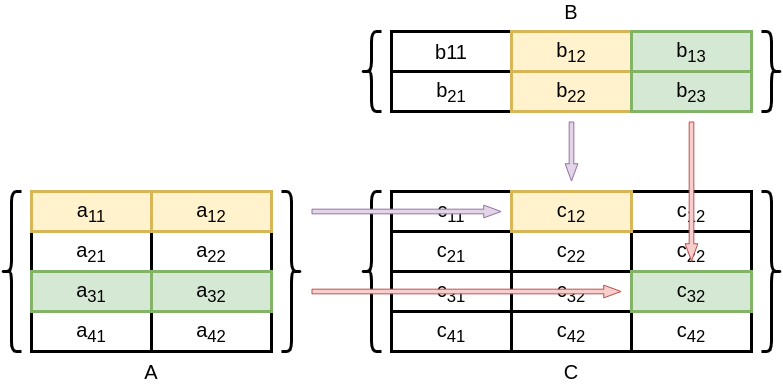
\includegraphics[scale=0.5]{l1.matrix}}
  \caption{Вычисление значения ячеек матрицы С}
  \label{ris:matrix}
\end{figure}

\section{Алгоритм Винограда}\label{Vinograd}

Алгоритм Винограда разработан на идее уменьшения количества операций умножений в цикле стандартного умножения матриц 
с помощью предварительной обработки. Каждый элемент произведения матриц представляет собой скалярное произведение соответ
ствующих строки и столбца исходных матриц.

Рассмотрим скалярное произведение векторов 

$V = (v_1, v_2, v_3, v_4)$ и 
$W = (w_1, w_2, w_3, w_4)$

Вот оно:

{\centering
\begin{gather}
C = V W = v1  w1 + v2  w2 + v3  w3 + v4  w4 =\\
(v1+w2) (v2+w1) + (v3+w4)  (v4+w3) \underbrace{- v1  v2 - v3 v4 - w1 w2 - w3 w4}_{\text{Можно вычислить заранее}}
\end{gather}\label{formula:multiplicatevectors}}

Несмотря на то, что конечный вариант формулы (\ref{formula:multiplicatevectors}) выглядит громоздко, и в нем целых 
6 операций умножения вместо 4. Однако последние 4 операции можно вычислить заранее. Тогда над обработанными данными
надо будет выполнять только 2 умножения и 5 сложений (и еще 2 сложения, чтобы добавить вычисленные заранее данные).

\section{Вычисление трудоемкости}\label{Complexity}

В данной работе необходимо расчитать трудоемкость исследуемых алгоритмов.
Будет использоваться следующая модель вычислений:

\begin{enumerate}
  \item Операции, трудоемкость которых равна 1: =, +, -, ++, --, +=, -=, <=, >=, ==, !=, [ ], <<, >>
  \item Операции, трудоемкость которых равна 2: *, /, *=. /=, \%, \%=
  \item Трудоемкость условного перехода равна 1.
  \item Трудоемкость цикла равна 
  
  $f_{for} = f_{init} + f_{comp} + N\cdot(f_{inc} + f_{comp} + f_{body})$
\end{enumerate}

\section{Вывод аналитической части}\label{End_analis_chapter}

В данной работе стоит задача реализации следующих алгоритмов: стандартного алгоритма умножения матриц, алгоритма Винограда 
и задача оптимизации алгоритма Винограда. Необходимо сравнить алгоритмы умножения матриц по эффективности по времени.
Подтвердить эффективность оптимизированного алгоритма Винограда.
 

